\documentclass[a4paper]{article}

\usepackage{enumerate}%used for custom enumerates
\usepackage{amsmath}%Math package
\usepackage{amssymb}%Math Package
\usepackage[utf8]{inputenc}%for the umlaut
\usepackage[german]{babel}%localized string of Chapter and other keywords
\usepackage{framed}%Framed used for the definitions
\usepackage{tabularx}%needed for the tebles environment
\usepackage{tikz}%used to draw all of the graphs
\usetikzlibrary{arrows}%custom arrows for chapter 1
\usepackage{pgfplots}%used for drawn graphs, for the figures
\usepackage{xcolor}%Color package, used for some diagrams
\usepackage{romanbar}%Used for chapter one for the X with over and underline
\newcolumntype{Y}{>{\centering\arraybackslash}X}%Used to center the text in the columns
\usepackage{fancyhdr}%Styling package used to dispaly custom headers, as well as custom chapter numbering in page numbering
\usepackage{float}%Used to position images in specified places
\pgfplotsset{compat=newest}%used for the pgfplots
\usetikzlibrary{decorations.pathmorphing,patterns}
\usepackage[bookmarks,bookmarksdepth=2]{hyperref}%Depth of index in pdf program
\usetikzlibrary{calc} %required for cube drawing in chapter 2
\usetikzlibrary{patterns,decorations.pathreplacing}%required for underbrace in tikz

% THESE PACKAGES ARE EDITING HELPERS, PROVIDING TOOLS FOR WHEN EDITING. THEY CAN BE DISABLED WHEN DONE
%\usepackage{showframe}%used to show margins in the preview, deactivate at the end
\usepackage{verbatim}%used for multiline comments, can be removed at the end
\usepackage{todonotes}%Notes to add throughout the document%PAckages file, can be found in Others/Packages.tex
\newenvironment{definition}[1]{\begin{framed}\centerline{\textbf{Definition #1}}\noindent\hspace{-1.1mm}}{\end{framed}}
\newenvironment{beweis}[1]{\subsubsection*{Beweis #1}}{\begin{flushright}$\blacksquare$\end{flushright}}
\DeclareMathOperator{\arccosh}{arccosh}%Defined here since it doesn't exist
\DeclareMathOperator{\arcsinh}{arcsinh}%Defined here since it doesn't exist
\DeclareMathOperator{\arctanh}{arctanh}%Defined here since it doesn't exist
\newcommand{\verteq}[0]{\begin{turn}{90} $=$\end{turn}}%added vertical equal sign
\DeclareMathOperator{\Hess}{Hess}%Defined here since it doesn't exist%custom environments, still in BETA
\pagestyle{fancy}

\fancyhf{}
\fancyhead[LE,RO]{}
\fancyhead[LO,RE]{\slshape \leftmark}
\fancyfoot[C]{\thepage}
\renewcommand{\headrulewidth}{0pt}

%Extra!
\usepackage{makeidx}
\usepackage{graphicx}
\usepackage{amsthm}

\makeatletter
\fancypagestyle{plain}{%
  \fancyhf{}
  \if@mainmatter
    \fancyfoot[C]{\thepage}
  \else
    \fancyfoot[C]{\thepage}
  \fi
  \renewcommand{\headrulewidth}{0pt}
}
\makeatother
\begin{document}
\setcounter{page}{0}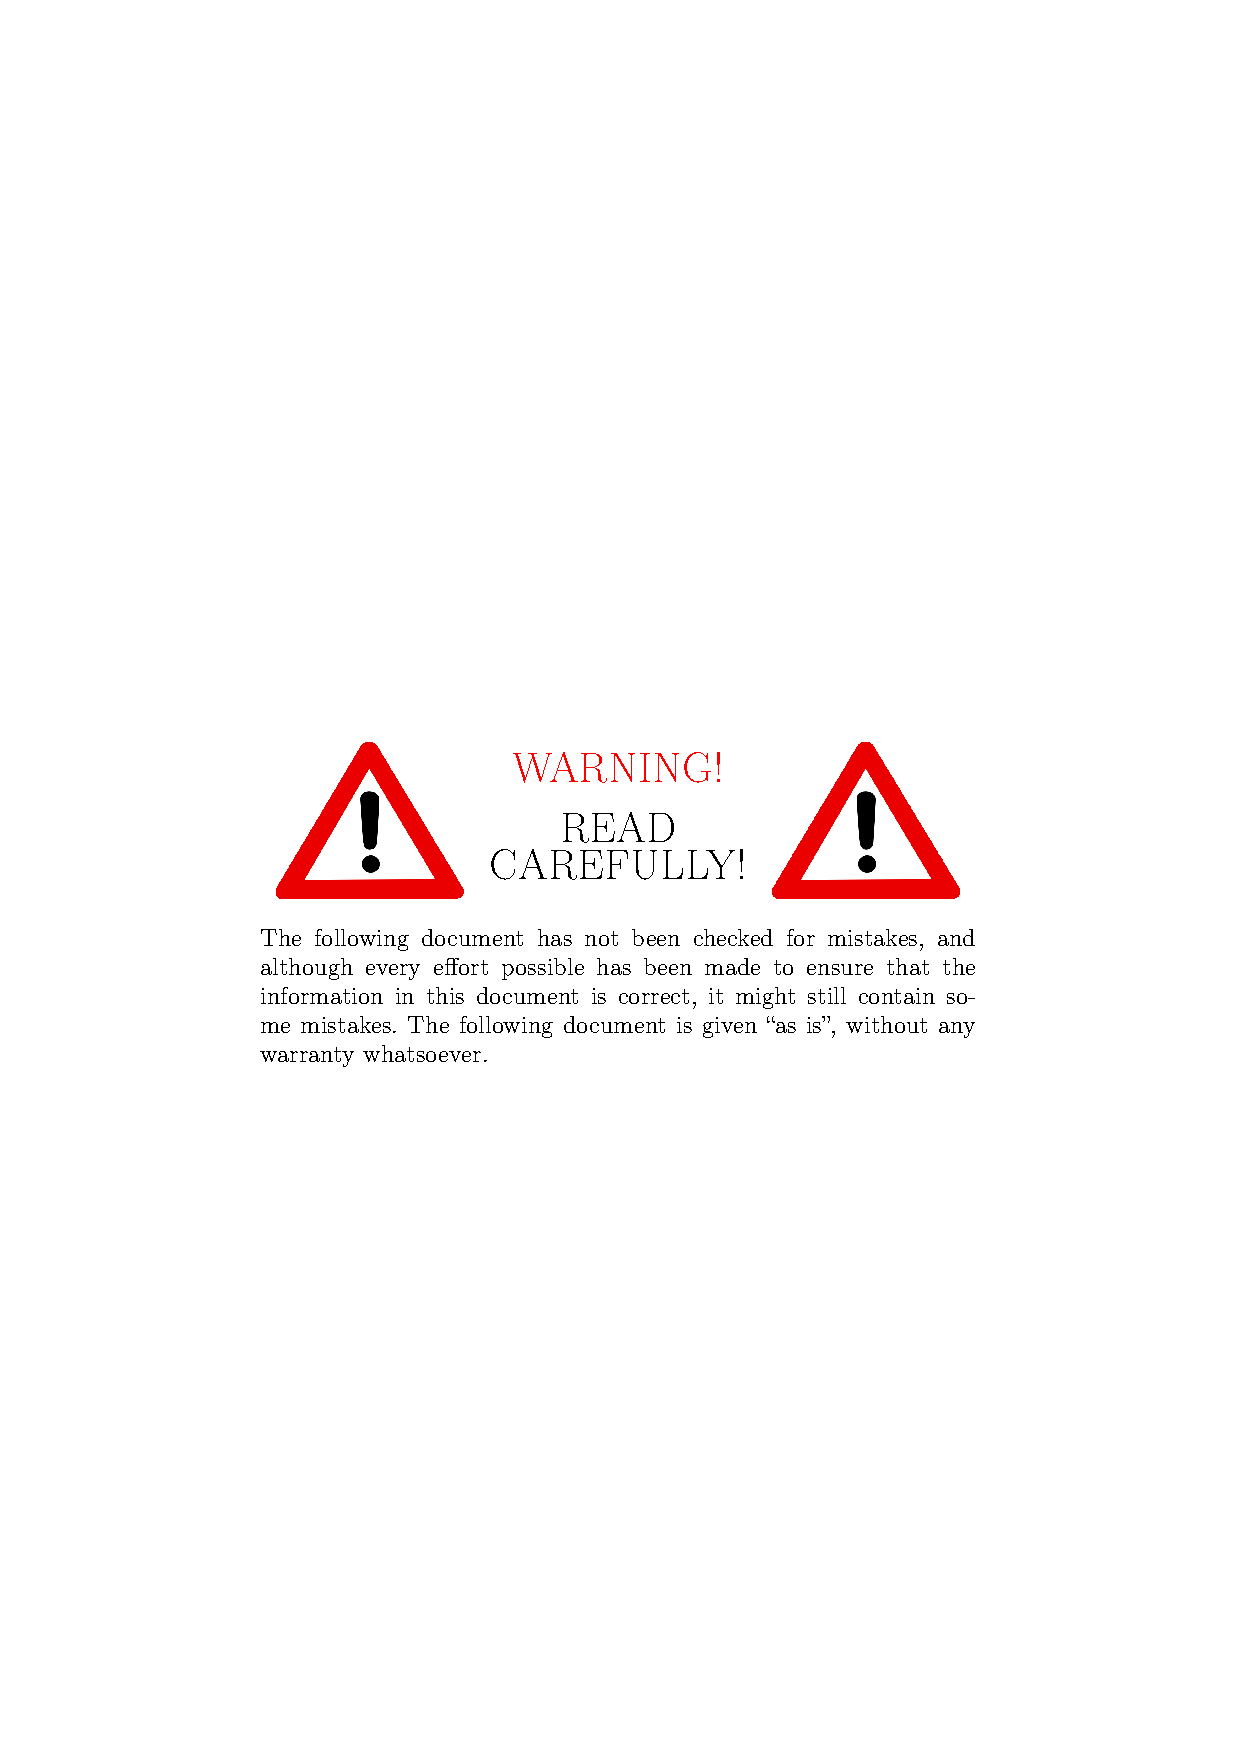
\includepdf[pages=-]{../Others/warningTex.pdf}
\section{Integration}
Let $f:\R\to\R$ be a continuous function, $P=\left\{ a=x_0<x_1<\dots <x_n<b\right\}$ a partition of the interval $\lbrack a,b\rbrack$ and $\xi_k\in\left[ x_k,x_{k+1}\right]$ points in each subinterval, then the sum 
\[S\left( {f,P,\xi } \right) = \sum\limits_{k = 0}^{n - 1} {\left( {\mathop {\inf }\limits_{{I_k}} f} \right)\left( {{x_{k + 1}} - {x_k}} \right)} \]
is called the Reimann sum \todo{?? attached ?? page 1 middle} to $f$ and to \todo{Chopped content, page 1 middle}
\begin{align*}
U(f,P)&:=\sum\limits_{k = 0}^{n-1} {(\mathop {{\text{inf }}f}\limits_{I_k} )} ({x_{k+1}} - {x_{k}})\\
O(f,P)&:=\sum\limits_{k = 0}^{n-1} {f(\mathop {{\text{sup}}f}\limits_{I_k} )} ({x_{k+1}} - {x_{k}})
\end{align*}
(where $I_k=\left[x_k,x_{k+1}\right]$) are called the lower \& upper Riemann sums. Similarly
\[\int\limits_{\underline{a}}^{b} {fdx = \sup\left\{ {U\left( {f,P} \right),P \in P} \right\}} \]\todo{Chopped content, page 1 middle to bottom} 
and
\[\int\limits_a^{\overline{b}} {fdx = \inf \left\{ {O\left( {f,P} \right),P \in P} \right\}} \]
are called lower and upper Integrals of $f$. $f$ is called Riemann integrable if 
\[\int\limits_{\underline{a}}^b {fdx = } \int\limits_a^{\overline{b}} {fdx} \]
\begin{fact}{}
\begin{enumerate}
\item Each continuous function is Riemann integrable
\item Each monotone function is Riemann integrable
\end{enumerate}
\end{fact}
\subsubsection*{Properties}
Let $f,g$ Riemann integrable on $I$, $\alpha,\beta\in\R$ for
\begin{enumerate}
\item \[\int\limits_a^b {\left( {\alpha f + \beta g} \right)dx}  = \alpha \int\limits_a^b {fdx}  + \beta \int\limits_a^b {gdx} \]
\item if $f(x)\leq g(x)$, $\forall x\in\lbrack a,b\rbrack$ then \[\int\limits_a^b {fdx}  < \int\limits_a^b {gdx} \]
\item \[\left| {\int\limits_a^b {f(x)dx} } \right| \le \int\limits_a^b {\left| {f(x)} \right|dx} \]
\item \[\left( {\mathop {\inf }\limits_I f} \right)\left( {b - a} \right) \le \int\limits_a^b {f(x)dx}  \le \left( {\mathop {\sup }\limits_I f} \right)\left( {b - a} \right)\]
\item \[\int\limits_a^b {fdx}  =  - \int\limits_b^a {fdx} \]
\item \[\int\limits_a^b {fdx}  = \int\limits_a^c {fdx}  + \int\limits_c^b {fdx},\hspace{5mm}\forall a,b,c\in\R \]
\end{enumerate}

\begin{fact}{(MWS der Integralrechnung)}
$f:\lbrack a,b\rbrack\to\R$ continuous, then $\exists \rho\in (a,b)$
\[\int\limits_a^b f(x) dx=f(\rho)(b-a)\]
\end{fact}


\begin{fact}{(Fundamental \todo{Can't read, page 3 middle to top} of calculus)}
\begin{enumerate}
\item Let $f:\lbrack a,b\rbrack\to\R$ continuous. Define 
\[F(x): = \int\limits_a^x {f\left( t \right)dt}\hspace{5mm} \forall x \in \left[ {a,b} \right]\]
then $F$ is differentiable and $F'=f$. $F$ is called primitive (Stammfunktion) of $f$.
\item If $G$ is \todo{Can't read, page 3 middle to bottom} primitive of $f$, then $G=F+c$ for some constant
\item Let $F$ be \todo{?? any ?? page 3 middle to bottom} primitive of $f$ then \[\int\limits_a^b f(x)dx=F(b)-F(a)\]
\end{enumerate}
\end{fact}

\subsection*{How do we calculate integrals?}
\begin{enumerate}
\item \textbf{Partial Integration:} Follows from product rule for differentiation
\begin{align*}
\int f(x) g'(x) dx =& f(x)g(x) - \int f'(x) g(x) dx\\
\int\limits_a^b f(x) g'(x) dx =& \left.f(x)g(x)\right|_a^b - \int\limits_a^b f'(x) g(x) dx\\
\end{align*}
\item \textbf{Substitution:} It follows from chain rule for differentiation
\begin{align*}
\int f(x) dx =&\int f\left(\varphi(y)\right) \varphi'(y) dy\\
\int\limits_{\tilde{a}}^{\tilde{b}} f(x)  dx =&\int\limits_a^b f\left(\varphi(y)\right) \varphi'(y) dy\\
\end{align*}
where $\varphi(a)=\tilde{a}$, $\varphi(b)=\tilde{b}$.
\item \textbf{Partialfractions:} To integrate rational functions of the form $\frac{P(x)}{Q(x)}$ with $P,Q$ polynomials. 
\begin{itemize}
\item If $\deg P < \deg Q$\\
We expand the rational function in simpler rational functions by finding the roots of $Q(x)$. Say \[Q(x)=(x-a_1){\dots}(x-a_n)\cdot\left( A_1x^2 + B_1x+C_1\right)\dots\left( A_nx^2 + B_nx+C_n\right)\]
Then for each linear factor $\left( x-a_i\right)$ of multiplication $r_i$ we need 
\[\frac{\alpha_{i1}}{\left( x-a_i\right)}+\frac{\alpha_{i2}}{\left( x-a_i\right)^2}+\dots+\frac{\alpha_{ir}}{\left( x-a_i\right)^r}\]
with constants $\alpha_{i1},\dots,\alpha_{ir}$. For each quadratic factor $A_ix^2+B_ix+C_i$ of multiply $S$ we have 
\[\frac{\beta_{i1}x+\gamma_{i1}}{A_ix^^2+B_ix+C_i}+\dots+\frac{\beta_{iS_i}x\gamma_{iS_i}}{A_ix^^2+B_ix+C_i}\]
witch constants $\beta_{ij},\gamma_{ij}$, $j=1,\dots,S$.
\item If $\deg P \geq \deg Q$\\
We first do long division to unite
\[\frac{P}{Q}\cdot R(x) + \frac{\tilde{P}(x)}{{Q}(x)}\]
with polynomials $R(X)$ and $\tilde{P}(x)$ with $\deg \tilde{P}<\deg$\todo{Chopped content page 5 midde to bottom}. Proceed as in the first case
\end{itemize}
\todo[inline]{Can't understand 1 word out of two, last paragraph in page 5}
\end{enumerate}
\subsubsection*{Beispiel}
Berechne 
\begin{enumerate}
\item \[\int\limits_1^2\frac{\sqrt{1+\ln(x)}}{x}dx\]
\item \[\int \cos(x)\cosh(x) dx\]
\item \[\int\frac{x^2-x+2}{x^3-x^2+x-1}dx\]
\end{enumerate}
\subsubsection*{Solution}
\begin{enumerate}
\item Note $\frac{1}{x}$ is the derivative of $\left( \ln(x)+1\right)$. Hence using substitution $u=\left( 1+\ln(x)\right)\Rightarrow du = \frac{1}{x}dx$
\[\int\limits_1^2 \frac{\left( 1+\ln(x)\right)^{\frac{1}{2}}}{x}dx=\int\limits_1^{1+\ln(2)} u^{\frac{1}{2}}du = \left.\frac{u^{\frac{3}{2}}}{\frac{3}{2}}\right|^{1+\ln(2)}_1=\frac{2}{3}\left[  \left(1+\ln(2)\right)^{\frac{3}{2}}-1\right]\]
\item This one is suitable for Integral by parts:
\begin{align*}
I &= \int {\underbrace {\cos (x)}_u\underbrace {\cosh (x)}_{v'}} dx\hspace{10mm}
\boxed{\begin{aligned}
u &= \cos (x)  	&&v'=  \cosh (x)\\
u' &=  - \sin (x)  &&v= \sinh (x)
\end{aligned}}\\
I &= \cos (x)\sinh (x) + \int {\underbrace {\sin (x)}_u\underbrace {{\mathop{\rm sinhh}\nolimits} (x)}_{v'}} dx\hspace{10mm}
\boxed{\begin{aligned}
u &= \sin (x)  	&&v'=  \sinh (x)\\
u' &=  \cos (x)  &&v= \cosh (x)
\end{aligned}}\\
I &=\cos(x)\sinh(x)+\left[ \sin(x)\cosh(x) - \int \cos(x)\cosh(x) dx\right]\\
I&=\cos(x)\sinh(x)+\sin(x)\cosh(x)-I\\
2I&=\cos(x)\sinh(x)+\sin(x)\cosh(x)\\
x&=\frac{1}{2}\left( \cos(x)\sinh(x)+\sin(x)\cosh(x)\right) + C
\end{align*}
\item \[\int\frac{x^2-x+2}{x^3-x^2+x-1}dx\]
Note: $x^3-x^2+x-1 = x^2(x-1)+(x-1) = (x^2+1)(x-1)$
\begin{align*}
\frac{x^2-x+2}{x^3-x^2+x-1}=\frac{A}{x-1}+\frac{Bx+C}{x^2+1}&=\frac{1}{x-1}-\frac{1}{x^2+1}\\
A(x^2+1)+(x-1)(Bx+C) &= x^2-x+2
\end{align*}
\begin{align*}
x=1&\Rightarrow 2A=2\Rightarrow A=1\\
x=2&\Rightarrow 5+2B+C=4\Rightarrow 2B+C = -1\\
x=0&\Rightarrow 1-C=2\Rightarrow C=-1\\
&\Rightarrow B=0
\end{align*}
\[\Rightarrow\int\frac{x^2-x+2}{x^3-x^2+x-1}dx = \ln\abs{x-1}-\tan^{-1}(x)+C \]
\end{enumerate}

\subsection*{Improper Integrals}
The improper integral of an integrable function $f$ on $(a,b)$ which is integrable on any subinterval $\lbrack a',b'\rbrack$ we define the improper integral as 
\[\int\limits_a^b {f(x)dx: = \mathop {\lim }\limits_{a' \searrow a} \mathop {\lim }\limits_{b' \nearrow b} } \int\limits_{a'}^{b'} {f(x)dx} \]
\subsubsection*{Example (Basisprüfung Frühling 2010)}
Untersuche ob das uneigentliche Integral $\int\limits_1^{\infty}\frac{1}{x^2+x}dx$ konvergiert. Falls ja, berechne den Wert. \\

\noindent Note: since $\frac{1}{x^2+x}<\frac{1}{x^2}$ and $\int\limits_1^{\infty}\frac{1}{x^2}dx$ is convergent, so is $\int\frac{1}{x^2+x}$
\begin{align*}
\int\frac{1}{x^2+x}&=\int\left( \frac{1}{x}-\frac{1}{x+1}\right)dx\\
&=\ln\abs{x}-\ln\abs{x+1} = \ln\abs{x\over{x+1}}
\end{align*}

\begin{align*}
\int\limits_1^{\infty}\frac{1}{x^2+x}&=\lim\limits_{b\to\infty}\int_1^b\frac{1}{x^2+x}dx\\
&=\lim\limits_{b\to\infty} \ln\abs{x\over{x+1}}_1^b\\
&=\lim\limits_{b\to\infty} \ln\left( \frac{b}{b+1}\right) - \ln\left( \frac{1}{2}\right)\\
&=\ln(1)+\ln(2)=\ln(2)
\end{align*}
limit exists and is equal to $\ln(2)$

\begin{fact}{}
\begin{enumerate}
\item \[\forall s\in\R, a>0, \int\limits_{a}^\infty\frac{dx}{x^s}=\begin{cases}\frac{a^{1-s}}{s-1} & s>1\\\infty & s\leq 1  \end{cases}\]
\item If $f$ is in $\lbrack a,\infty)$ continuous, and $\exists c$ and $s>1$ so that $\abs{f(x)}\leq\frac{c}{x^s}$, $\forall x\geq a$, then $\int\limits_a^\infty f(x)dx$ converges (Majorantenkriterium)
\item If $f$ is in $\lbrack a,\infty)$ continuous, and $\exists c>0$ \todo{Can't understand, page 9 bottom}$f(x)\geq\frac{c}{x},\forall x\geq a$, then $\int\limits_a^\infty f(x)dx$ diverges to $\infty$.
\end{enumerate}
\end{fact}

\subsubsection*{Example}
\begin{align*}
&\int\limits_1^\infty \frac{t^2+4}{\left( 1+4t^2\right)^{\frac{3}{2}}}\text{ diverges}\\
&\int\limits_1^\infty \frac{t^2+4}{\left( 1+4t^2\right)^{\frac{5}{2}}}\text{ converges}
\end{align*}
Because
\[\text{if $t$ is large enough, say $t>2$}\begin{cases}t^2<t^2+4<2t^2\\ 4t^2<1+4t^2<5t^2\end{cases}\]
Hence
\begin{align*}
\frac{t^2}{(5t)^{2\alpha}} < & \frac{t^2+4}{\left( 1+4t^2\right)^\alpha} < \frac{2t^2}{\left( 4t\right)^{2\alpha}}\\
\frac{C_1}{(t)^{2\alpha-2}} < & \frac{t^2+4}{\left( 1+4t^2\right)^\alpha} < \frac{C_2}{\left( 4t\right)^{2\alpha-2}}
\end{align*}
$\Rightarrow$ if $\alpha = \frac{3}{2}$
\[\frac{t^2+4}{\left( 1+4t^2\right)^{\frac{3}{2}}}>\frac{C_1}{t}\]
And since $\int\limits_1^{\infty}\frac{dt}{t}$ diverges, so does \[\int\limits_1^\infty\frac{t^2+4}{\left( 1+4t^2\right)^{\frac{3}{2}}}dt\]
Similarly since for $\alpha=\frac{5}{3}: 2\alpha-2=\frac{10}{3}-2>1$ and 
\[\int\frac{C_2}{t^{\frac{4}{3}}}dt\]
converges, so does
\[\int\frac{t^2+4}{\left( 1+4t^2\right)^{\frac{5}{3}}}dt<\int\frac{C_2}{t^{\frac{4}{3}}}dt\]

\section{Differential Equations}
\subsection{Linear Differential equations with constant coefficients}
To solve a linear differential equation of the form $Ly = b(x)$, where
\[L:=\frac{d^n}{dx^n}+a_{n-1}\frac{d^{n-1}}{dx^{n-1}}+\dots+a_1\frac{d}{dx}+a_0\]
$b(x)$ a function, and $a_i\in\R$
\begin{enumerate}
\item Find a homogeneous solution $y_H$, namely a solution of $Ly=0$
\item Find a special solution $y_S$ of $Ly=b(x)$ using the method ``Ansatz von Typ der rechten Seite''
\item Then the general solution is given by \[y=y_H+y_S\]
\end{enumerate}
\subsubsection*{How to find the homogeneous solution $y_H$ of $Ly=0$}
\begin{enumerate}
\item Find the characteristic polynom of $L$, namely \[P_l(\lambda)=\lambda^n+a_{n-1}\lambda^{n-1}+\dots+a_1\lambda+a_0\]
\item \begin{fact}{}
If $\lambda_1,\dots,\lambda_{r\in\C}$ are the Pairwise distinct roots of $P(\lambda)=0$ with associated multiplicates $m_1,\dots,m_r$, then the functions
\[x\to x^ke^{\lambda_jx}, 1\leq k\leq r,0\leq k\leq m_j\]
Form a system of fundamental solutions of the homogeneous equations $Ly=0$
\subsubsection*{Variant\todo{Not really sure if it says variant, page 13 middle to bottom}}
If $L$ has  real coefficients, every pair of complex, non-real roots $\lambda_j = \mu_j\pm iv_j$ of multiply $m_j$ give a fundamental solution 
\[k^ke^{\left( \mu_j\pm iv_j\right)x} = x^ke^{\mu_j}\left( \cos(v_jx)\pm i\sin(v_jx)\right)\]
for $0\leq k<m_j$. So one can, as a basis, take
\[x^ke^{\mu_j x}\cos v_j x\text{ and }x^ke^{\mu_j x}\sin v_j x\]
instead of 
\[x^ke^{(\mu_j + iv_j)x} \text{ and }x^ke^{(\mu_j-iv_j)x}\]
Then the general homogeneous solution is of the form 
\[y_H(x)=\sum\limits_{j=1}^r\sum\limits_{k=0}^{m_j}c_{jk}x^ke^{\lambda_jx}\]
with constant $c_{jk}$
\end{fact}
\end{enumerate}

\subsubsection*{How to find the special solution of Inhomogeneous $Ly=b(x)$ using the method of ``Ansatz''}
\begin{fact}{}
\begin{enumerate}
\item Let $\lambda\in\C$. if $\lambda$ is not a solution of $P_L(\lambda)$, then the inhomogeneous DGL $Ly=e^{\lambda x}$ has particular solutions $y=\frac{1}{P_L(x)}e^{\lambda x}$
\item Let $\lambda\in\C$, $m$ its multiplicity as a solution of $P_L(\lambda)=0$ ($m$ can be zero, which means $\lambda$ is not a solution of $P_L(\lambda)=0$).\\

Let $Q(x)$ a polynomial of degree $k$. Then a particular solution of $Ly(x)=Q(x)e^{\lambda x}$ is of the form \[y(x)=R(x)e^{\lambda x}\] for a polynomial $R(x)$ of degree $k+m$
\item Let $l$ has a real coefficient. Let $\mu,v\in\R$, $m$ the multiplicity of $\mu\pm iv$ as a solution of $P_L(\lambda)=$\todo{Chopped contant, page 14 bottom} ($m=0$ means $\mu \pm iv$ is not a root of $P_L$). Let $Q(x)$ and $R(x)$ be polynomials of degree $\leq$\todo{Chopped content, page 15 top}. Then the particular solution of the inhomogeneous Differential equation 
\[Ly=Q(x)e^{\mu x}\cos vx +R(x)e^{\mu x}\sin x\]
is of the form 
\[y(x)=S(x(e^{\mu x}\cos vx + T(x)e^{\mu x}\sin x\]
for polynomials $S,T$ of degree $\leq k+m$
\end{enumerate}
\end{fact}
\subsubsection*{Boundary (Rand) or Initial value Problems (Anfangswert)}
When we are given a differential equation $Ly=b(x)$ together with either 
\begin{center}
\begin{tabular}{r c l}
Boundary values & or & Initial values\\
$y(a_1)=A_1$ & {} & $y(a)=A_1$\\
$y(a_2)=A_2$ & {} & $y'(a)=A_2$\\
\vdots\hspace{7mm} & {} & \hspace{7mm}\vdots\\
$y(a_n)=A_n$ & {} & $y^{(n-1)}(a)=A_n$\\
\end{tabular}
\end{center}
We first find the general solution $y=y_H+y_S$. Then we determine the constants $C_1,\dots, c_n$ in the homogeneous solution using the given boundary or initial values.

\subsubsection*{Example}
\begin{enumerate}
\item Basisprüfung Frühling 2011
\begin{enumerate}
\item Bestimme alle Lösungen $y=y(x)$ der DGL $y^{(4)}-y=0$ welche für $\abs{x}\to\infty$ beschränkt bleiben
\item Bestimme eine Lösung $y=y(x)$ der DGL $y^{(4)}-y=e^{-x}+x$
\end{enumerate}
\subsubsection*{Solution}
\begin{enumerate}
\item We first find the characteristic polynomial 
\begin{align*}
x^4-1=0\Rightarrow & \left( x^2-1\right) \left( x^2+1\right)=0\\
&\lambda = \pm 1,\lambda=\pm i
\end{align*}
The homogeneous solution is of the form 
\[y_H = C_1e^x+C_1e^{-x}+C_3\cos x+ C_4\sin x\]
Since 
\begin{align*}
e^x\to\infty&\text{ as }x\to\infty\\
e^{-x}\to\infty&\text{ as }x\to-\infty
\end{align*}
The solutions that satisfy \todo{Can't read, page 16 bottom} are $y_H=C_3\cos x+C_4\sin x$ with $C_3,C_4\in\R$
\item We use the superposition principle: Let $b_1(x)=e^{-x}, b_2(x)=x$
\begin{enumerate}
\item $y_{1S}$ is a solution of $Ly=b_1(x)$
\item $y_{2S}$ is a solution of $Ly=b_2(x)$
\end{enumerate}
Then $y_{1S}+y_{2S}$ is a solution of $Ly=e^{-x}+x$. Since $\lambda = -1$ is a root of $P_L(\lambda)=0$ of multiplicity, i.e. since $e^{-x}$ is also a solution of $Ly=0$\\

For $y_{1S}$ we take as ``ansatz'' $y_{1S}= Cxe^{-x}$. For $y_{2S}$ we take as ``ansatz'' $y_{2S}= Dx+E$ a polynomial of degree 1. So a special solution is of the form 
\[y_S = Cxe^{-1}+Dx+E\]
To find the constants $C,D,E,F$ we put this solution into the differential equation $y^{(4)}-y=e^{-x}+x$.
\begin{align*}
y'(x)&=C\left[e^{-x}-xe^{-x}\right]+D\\
y''(x)&=C\left[-e^{-x}-\left[e^{-x}-xe^{-x}\right]\right] = C\left[ -2e^{-x}+xe^{-x}\right]\\
y^{(3)}(x)&=C\left[2e^{-x}+\left[e^{-x}-xe^{-x}\right]\right] = C\left[3e^{-x}-xe^{-x}\right]\\
y^{(4)}(x)&=C\left[-3e^{-x}+\left[e^{-x}-xe^{-x}\right]\right] = C\left[-4e^{-x}+xe^{-x}\right]
\end{align*}
Then 
\begin{align*}
y^{(4)}_S-y_S(x) =& C\cdot 4e^{-x}+Cxe^{-x}-\left[ Cxe^{-x}+Dx+E\right]\\
\Rightarrow & 4Ce^{-x} -Dx-E = e^{-x}+x\\
\Rightarrow & 4C=1, D=-1
\end{align*}
Hence a particular solution is \[y_S=\frac{1}{4}xe^{-x}-x\]
General solution is 
\begin{align*}
y&=y_H+y_S\\
&=C_1e^x + C_2e^{-x}+C_3\cos x+C_4\sin x + \frac{1}{4}xe^{-x}-x
\end{align*}
\end{enumerate}
\item Basisprüfung Sommer 2013
\begin{enumerate}
\item Für welche Werte des Parameters $a\in\R$ strebt die allgemeine Lösung $y(x)$ der DGL $y''+2y'+ay=0$ unabhängig von den Anfangsbedingungen gegen 0 für $x=$\todo{Chopped content, page 18 bottom}
\item Finden Sie eine homogene DGL 2. ordnung mit konstanten Koeffizienten, deren allgemeine Lösung $y(x)=e^{-x}+2xe^{-x}$ ist. Was sind dann die Anfangsbedingungen bey $x=0$?
\end{enumerate}
\subsubsection*{Solution}
\begin{enumerate}
\item The characteristic polynomial of $y''+2y'+ay=0$ is $\lambda^2 + 2\lambda + a=0$. The roots are 
\[\lambda_{1,2}=\frac{-2\pm\sqrt{4-4a}}{2}=-1\pm\sqrt{1-a}\]
\begin{itemize}
\item If $1-a<0$ then there are 2 complex conjugate roots. Let $\abs{1-a}=b^2$ then the general solution is of the form 
\[y(x)=C_1e^{-x}\cos(bx)+C_2e^{-x}\sin(bx)\]
and this go to zero \todo{Can't read, page 19 middle} of $b$, hence $a$ since $e^{-x}$ decays to zero.
\item If $1-a=0$ then -1 is a double root. Then the solutions are of the form $C_1e^{-x}+C_2xe^{-x}$ and this will not decay to zero as $x\to\infty$
\end{itemize}
Similarly if $1-a>0$ then one of the roots will be positive if $\sqrt{1-a}>1$ and that root can lead to a growing solution. \\

Hence when $\sqrt{1-a}>1$, or $1-a>1$, or when $a<0$, then $-1+\sqrt{1-a}>0$, If on the other hang $0<a<1$ then again $1\pm\sqrt{1-a}<0$ and both solutions are decaying. Hence if $0<a<1$ or $a>1$ then the solutions is decaying \todo{Can't understand, page 20 middle to bottom} of initial values, and if $a=1$ or $a<0$ then the solution can be growing.
\item Let $Ly=0$ be of the form $y''+a_1y'+a_0=0$ then the characteristic polynomial is $\lambda^2+a_1\lambda +a_0$. Since we want $e^{-x}$ and $xe^{-x}$ to be the solutions, we should have $\lambda=-1$ with multiply 2, that means 
\[P_L(\lambda)=\lambda^2+2\lambda+1\]
and the differential equation is $y''+2y'+y=0$. The general solution of this equation is 
\[y_H=C_1e^{-x}+C_2xe^{-x}\]
Since the solution is $e^{-x}+2xe^{-x}$, $C_1=1$, $C_2=2$ we must have $y(0)=e^{-0}+2\cdot 0=1$
\[y'(0)=-e^{-x}+2\left.\left[ e^{-x}-xe^{-x}\right]\right|_{x=0} = -1+2=1\]
So we can choose $y(0)=1$, $y'(0)=1$
\end{enumerate}
\end{enumerate}

\subsection{Solving Differential Equations by separation of variables}
\subsubsection*{Example}
\begin{enumerate}
\item (Frühling 2011) Bestimme die Lösung $y=y(x)$ der DGL $y'=e^{x-y}$ mit $y(0)=0$
\subsubsection*{Solution}
\begin{align*}
&\hspace{7.7mm}\frac{dy}{dx}=e^x\cdot e^{-y}\\
&\Rightarrow e^y dy = e^x dx\\
&\Rightarrow \int e^y dx = \int e^x dx\\
&\Rightarrow e^y=e^x+C
\end{align*}
\todo{In my opinion there is an error, my solution (the same as Wolfram Mathematica) is $y(x)=\pm \sqrt{\frac{c+2x^3+6x}{3}}\frac{1}{x}$}
Since $y(0)=0\Rightarrow e^0 = e^0 + C\Rightarrow C=0$ and $y=x$
\item (Herbst 2010) Bestimme eine Lösung der DGL 
\[y+xy' = \frac{1}{y}\left( x+\frac{1}{x}\right), x>0\]
mit $y(1)=2$, $y(x)>0$, $\forall x$. (Hinweise: substituire $u(x)=xy(x)$).
\[u'(x)=y(x)+xy'(x)\]
Left hand side is
\begin{align*}
u'(x) &= \frac{x}{y}+\frac{1}{xy}=\frac{x^2}{u}+\frac{1}{u}=\frac{x^2+1}{u}\\
\Rightarrow \frac{u'}{u} &=x^2+1\Rightarrow \ln u = \frac{x^3}{3}+x+C\\
y(1)&=2 \Rightarrow u(1)=1\cdot y(1)=2\\
\Rightarrow \ln 2 &= \frac{1}{3}+1+C \Rightarrow C=(\ln 2)-\frac{4}{3}\\
u&=Ce^{\frac{x^3}{3}\cdot e^x}
\end{align*}
\end{enumerate}






%%%% INIZIO SANDRO
\subsection{Differentiation in many variables}
A function $f:\Omega \subset \R^n \rightarrow \R$ is (total) differentiable in $x_0$ if it exists a linear map $A:\R^n \rightarrow \R$ such that $$f(x)=f(x_0)+A(x-x_0)+R(x_0,x)$$
Where $\lim_{x\rightarrow x_0} \frac{R(x_0,x)}{|x-x_0|}=0$.
In this case A is called the differential of $f$ at $x_0$ and it's denoted as $(df)(x_0)$.

Let $(A_1, A_2, ... , A_n)$ be a matrix representation of the linear map $A:\R^n \rightarrow \R$ (wrt to the standard Basis). Then $f$ differentiable at $x_0$ means:
$$f(x)=f(x_0)+A_1(x^1-x_0^1)+A_2(x^2-x_0^2)+...+A_n(x^n-x_0^n)+R(x,x_0)$$

\[P(x,x_0)=f(x_0)+\begin{bmatrix}
A_1 & ... & A_n
\end{bmatrix} \begin{bmatrix}
x^1-x_0^1 \\ 
... \\ 
x^n-x_0^n
\end{bmatrix} \]
is the equation of the tangent plane at the point $f(x_0)$ on the surface formed by the graph of $f$.

\begin{fact}{}
if $f:\Omega \rightarrow \R$ is differentiable in $x_0 \in \Omega$ then the partial derivative exist and the differential $df(x_0)$ has the matrix representation $$\begin{pmatrix}
\frac{\partial f}{\partial x}(x_0) & ... & \frac{\partial f}{\partial x^n}(x_0) \end{pmatrix} = \nabla f$$ the gradient of $f$.
\end{fact}
\begin{fact}{}
$f$ differentiable in $x_0 \Rightarrow f$ is continuous in $x_0$.
\end{fact}
\begin{fact}{}
If all partial derivatives of $f$ are continuous then $f$ is differentiable
\end{fact}

Using these last two facts and the definition of differentiability one can study if a given function is differentiable or not. 

\subsubsection{Differentiation rules}
Let $f,g:\Omega \rightarrow \R$ be differentiable in $x_0$. Then:
\begin{enumerate}
\item $d(f\pm g)(x_0)=df(x_0)\pm dg(x_0)$
\item $d(fg)(x_0)=g(x_0)df(x_0)+f(x_0)dg(x_0)$
\item $d(f/g)(x_0)=\frac{g(x_0)df(x_0)-f(x_0)dg(x_0)}{(g(x_0))^2}$
\item Let $h:\R \rightarrow \R$ be differentiable in $g(x_0)$, then
$$d(h o g)(x_0)=h'(g(x_0))dg(x_0)$$
\item Let $H:I\subset \R \rightarrow \Omega \subset \R^n$ be differentiable in $t_0 \in \R$ and $f$ differentiable in $H(t_0)$. Then 
$$\frac{d}{dt} (f o H)(t_0)=df(H(t_0))H'(t_0)$$ where $H(t)=(H_1(t),...,H_n(t))$ and $H'(t)=(H_1'(t), ..., H_n'(t))$
\end{enumerate}

\subsubsection{Directional derivative}
The directional derivative of $f$ in the direction of a unit vector $e \in \R^n-\{0\}$ is given by 
$d_ef(x_0)=\nabla f(x_0) \cdot e$. 

\subsubsection{Particular higher derivatives}
One can similarly define higher derivatives order partial derivatives for functions $f \in C^m(\Omega)$.

\begin{fact}{(Schwarz)}
if $f \in C^2(\Omega)$ then $\frac{\partial^2 f}{\partial x^i \partial x^j}=\frac{\partial^2 f}{\partial x^j \partial x^i}$
and in general for $f \in C^m(\Omega)$ all $n$  partial derivatives of $f$ of order $\leq m$ are independent of the order of differentiation.
Using higher order derivatives one can analogous to the 1-dimensional case define a Taylor approximation of $f$.
\end{fact}

\begin{fact}{}
Let $f \in C^m(\Omega), f:\Omega \rightarrow \R, \Omega \in \R$ and $x_1,x_0 \in \Omega$. Then 
$$f(x_1)=f(x_0)+\nabla f(x_0)(x_1-x_0)+\frac{1}{2}\sum_{i,j=1}^2 \frac{\partial^2 f}{\partial x^i \partial x^j}(x_0)(x_i^i-x_0^i)(x_1^j-x_0^j) + R_3(f,x_1,x_0)$$ 
Where $\lim_{x_1 \rightarrow x_0} \frac{R(f,x_1,x_0)}{||x_1-x_0||}=0$
\end{fact}

The analogue of the second derivative is given by the matrix of partial derivatives of order 2. This matrix is called the Hesse-matrix of $f$.
$$\Hess(f)=\nabla^2 f=\left(\frac{\partial^2 f}{\partial x^i \partial x^j}\right)_{i,j=1,...,n}$$

\subsubsection{The extrema of a function $f:\Omega \rightarrow \R$}
\begin{definition}{}
A point $x \in \Omega$ is called a critical point if $\nabla f(x)=0$.
\end{definition}
\begin{fact}{}
$f$ differentiable, $x_0$ is called local extrema of $f$ then $x_0$ is a critical point
\end{fact}
\begin{fact}{}
Let $x_0$ be a critical point of $f$. Then we have three different cases:
\begin{enumerate}
\item $x_0$ is a local minima if $\nabla^2 f(x_0)$ is positive definite.
\item $x_0$ is a local maxima if $\nabla^2 f(x_0)$ is negative definite.
\item Otherwise it is a saddle point (Sattelpunkt).
\end{enumerate}
\end{fact}

\begin{fact}{}
Let $f:\Omega \rightarrow \R$ be continuous and differentiable on an open set $\Omega \subset \R^n$. Let $\partial \Omega$ be the boundary of $\Omega$. Then every global extrema of $f$ is either a critical point of $f$ in $\Omega$ or a global extremal point of $f|_{\partial \Omega}$ (f restricted to the boundary)
\end{fact}

\subsubsection*{Example (FS 2011)}
Sei $f(x,y)=4x^2y^2-x^2-4y^2+1$. Bestimme die globalen Extrema von $f$ auf dem Gebiet $\Omega=\{(x,y)=\frac{x^2}{4}+y^2\leq 1, y\geq0\}$.
\subsubsection*{Solution}
We first find the critical points:
$$\nabla f=\begin{pmatrix} 8xy^2-2x \\ 8x^2y-8y \end{pmatrix} =  \begin{pmatrix}
0 \\ 
0
\end{pmatrix} $$
\begin{align*}
2x(4y^2-1)=0 \Rightarrow & x=0 \mbox{ or } y=\pm \frac{1}{2} \\
8y(x^2-1)=0 \Rightarrow & x=\pm 1 \mbox{ or } y=0
\end{align*}
$(0,0), (\pm 1, \pm \frac{1}{2})$ are the critical points of $f$. Since $y\geq 0$ we only take $P_1=(0,0), P_{2,3}=(\pm 1, \frac{1}{2})$. Then we need to compute $\Hess(f)$.
$$\Hess(f)=\begin{pmatrix}
8y^2-2 & 16xy \\ 
16xy & 8x^2-8
\end{pmatrix} $$
$$\Hess(f)(0,0)=\begin{pmatrix}
-2 & 0 \\ 
0 & -8
\end{pmatrix} \Rightarrow \mbox{ negative definite } \Rightarrow \mbox{ local maxima}$$ 
$$\Hess(f)(1,\frac{1}{2})=\begin{pmatrix}
0 & 8 \\ 
8 & 0
\end{pmatrix} \Rightarrow \mbox{ indefinite }$$ 
$$\Hess(f)(-1,\frac{1}{2})=\begin{pmatrix}
0 & -8 \\ 
-8 & 0
\end{pmatrix} \Rightarrow \mbox{ indefinite }$$ 
To find global extrema we need to look at $f$ on the boundary of $\Omega$, which is the curve $\frac{x^2}{4}+y^2=1$ and the line $y=0$. First on the line $y=0$ let $g=f|_{y=0}=-x^2+1$. $$g'(x)=-2x \Rightarrow x=0, P_1(0,0) \mbox{ is a point we need to check}$$
We also need to check the corners $P_{4,5}=(\pm 2,0)$. On the ellipse: let $h=f|_{\frac{x^2}{4}+y^2=1}=-x^4+4x^2-3$.
$$h'(x)=-4x^3+8x=0 \Rightarrow P_6=(0,1), P_{7,8}=(\pm \sqrt{2}, \frac{1}{\sqrt{2}})$$
Now we look at the values of $f$ at these points. $f(P_1)=f(0,0)=1, f(P_{2,3})=0, f(P_{4,5})=-3, f(P_6)=-3, f(P_{7,8})=1$. $f$ has also a minima at $(\pm 2,0), (0,1)$ and a maxima at $(0,0), (\pm \sqrt{2}, \frac{1}{\sqrt{2}})$.

\subsubsection*{Example (FS 2010)}
\begin{enumerate}
\item Bestimme das Taylorpolynom erster Ordnung der Funktion $f(x,y)=e^{x^2}(x+y)$ um dem Punkt $(1,1)$.
\item Bestimme $c \in \R$ so dass der Vektor $\begin{pmatrix}
1 \\ 
-1 \\ 
c
\end{pmatrix} $ tangential an den Graphen $g(f)=\{(x,y,f(x,y)):(x,y)\in \R^2$ im Punkt $(1,1,z)$ liegt.
\end{enumerate}
\subsubsection*{Solution}
\begin{enumerate}
\item
$$\nabla f=\begin{pmatrix}
2xe^{x^2}(x+y)+e^{x^2} \\ 
e^{x^2}
\end{pmatrix}, \nabla f(1,1)=\begin{pmatrix} 5e \\ e \end{pmatrix}, f(1,1)=2e$$
\begin{align*}
f(x,y)&=2e+\begin{pmatrix} 5e \\ e \end{pmatrix}(x-1,y-1)+r_2(x,y)\\
&=2e+5e(x-1)+e(y-1)+(x-1)(\nabla^2 f)(t)\begin{pmatrix} x-1 \\ y-1 \end{pmatrix}
\end{align*}
The Taylor polynomial of order 1 is $z=2e+5e(x-1)+e(y-1)$
\item The vector $(1, -1, c)^T$ must be perpendicular to the normal vector of the plane, that is (from part 1) $n=(5e, e, -1)^T$. Hence
$$(1, -1, c) \cdot (5e, e, -1)=0 \Rightarrow 4e-c=0 \Rightarrow c=4e$$
\end{enumerate}

\subsection{Line (Weg) integral}
Let $v:\Omega \rightarrow \R^n$ be a vector field and $\gamma$ a curve with parametrization $\gamma: [a,b]\rightarrow \Omega, t\rightarrow \gamma(t)$. Then the line integral of $v$ along $\gamma$ is defined as 
$$\int_{\gamma} v ds= \int_a^b <v(\gamma(t)),\gamma '(t)> dt$$

\subsubsection*{Facts}
\begin{enumerate}
\item $\int_{\gamma} vds$ is independent of the parametrization of the path.
\item $\int_{\gamma_1+\gamma_2} vds=\int_{\gamma_1} vds+ \int_{\gamma_2} vds$
\item $\int_{\gamma} vds= -\int_{-\gamma} vds$
\item If v  is the gradient vector field associated to a function $f$ i.e. $v=df$ then $\int_{\gamma} vds=f(\gamma(b))-f(\gamma(a))$, where $\gamma: [a,b] \rightarrow \Omega$.
\end{enumerate}
Equivalent one can change everything in terms of 1-forms $\lambda=\lambda_1 dx^1+\lambda_2 dx^2+ ... + \lambda_n dx^n$. Then $$\int_{\gamma} \lambda = \int_a^b \lambda(\gamma(t))\gamma '(t)dt$$

\begin{fact}{}
$\lambda: \Omega \rightarrow L(\mathbb{R^n}, \R)$ a constant 1-form, then the following are equivalent:
\begin{enumerate}
\item $\exists f \in C'(\Omega) : df=\lambda$
\item For every 2 continuous C'-paths $\gamma_1, \gamma_2$ with $\gamma_i:[a_i,b_i]\rightarrow \Omega$ with the same beginning and ending points:
$$\int_{\gamma_1} \lambda=\int_{\gamma_2} \lambda$$
\item For every closed curve $\gamma$, $\int_{\gamma}=0$
\end{enumerate}
\end{fact}
\begin{definition}{}
A vector field $V:\Omega \rightarrow \R^n$ is called conservative if $\int_{\gamma} Vds=0$ for every closed curve $\gamma$.
\end{definition}

\begin{fact}{}
For a simply connected region $\Omega$, we have
$$\mbox{ V is conservative } \iff v=\nabla f \mbox{ for some function } f$$
\end{fact}

\subsubsection*{Example (FS 2010)}
Berechne das Wegintegral $\int_\gamma vds$ entlang das eingezeichneten Weg für das Vektorfeld $v(x,y)=\begin{pmatrix}
xy^2 \\ 
-y
\end{pmatrix} $
\begin{center}
\begin{tikzpicture}[scale= 0.5]
\draw[->](-0.5,0) --(6,0);
\draw[->](0,-3.5) --(0,6);

\draw[very thick,->] (0,3) -- (0,1.5);
\draw[very thick] (0,1.5) -- (0,0); 

\draw[very thick] (4,5) -- (4,2.5);
\draw[very thick,<-] (4,2.5) -- (4,0); 

\draw[very thick] (4,5) parabola bend (0,3) (0,3); 
\draw[very thick,<-] (2,3.5) -- (2.01,3.505);

\draw[very thick, ->] (0,0) --(2,-1.5);
\draw[very thick] (2,-1.5) -- (4,-3);


\draw(4,2.8) node [anchor=west]{$\gamma_1$};
\draw(2,4) node [anchor=east]{$\gamma_2$};
\draw(0,1.8) node [anchor=east]{$\gamma_3$};
\draw(2,-2) node [anchor=east]{$\gamma_4$};

\draw(4,0.2) -- (4,-0.2) node[anchor = north] {1};
\draw(0.2,3) -- (-0.2,3) node[anchor = east] {1};
\draw(0.2,-3) -- (-0.2,-3) node[anchor = east] {1};

\draw (3.5,4.5) parabola bend (4.5,5.5)(4.5,5.5) node[anchor = west]{$y=e^x$};

\end{tikzpicture}
\end{center}
\[\int_\gamma vds=\int\limits_{\gamma_1+\gamma_2+\gamma_3+\gamma_4} vds\]

\subsubsection*{Solution}
We first parametrize the curves:
\begin{enumerate}
\item $\gamma_1=(1,t), t \in [0,e] \Rightarrow \gamma_1 '=(0,1)$
\item $-\gamma_2=(t,e^t), t \in [0,1] \Rightarrow -\gamma_2 '=(1, e^t)$
\item $\gamma_3=(0,1-t), t\in [0,1] \Rightarrow \gamma_3 '=(0,-1)$
\item $\gamma_4=(t,-t) t\in [0,1] \Rightarrow \gamma_4 '=(1,-1)$
\end{enumerate}
$$\int_{\gamma} vds= \int_0^e (t^2, -t)\cdot(0, 1)dt+\int_1^0(te^{2t}, -e^t)\cdot (1, e^t)dt + ...$$
See the last example of Green's theorem for the rest.

\subsection{Integration in $\R^n$}
The Riemann integral in $\R^n$ is constructed in analogue way to the case in n=1. With Riemann sums over subintervals is replaced with sums over "sub-rectangles". $dx$ is replaced with an n-dimensional volume element $dvol_n$ which we denote also by $d\mu(x)$.
\begin{fact}{}
For a normal-region $$D=\{(x,y) \in \R^2 : a\leq x\leq b, \phi (x)<y< \psi (x)\}$$
Where $\phi, \psi$ are continuous functions: $\R \rightarrow \R$ we have
$$\int_D fd\mu(x)= \int_a^b \int_{\phi(x)}^{\psi(x)} f(x,y) dy dx$$ 
\end{fact}

\begin{fact}{}
For a rectangle $Q=[a,b]\times[c,d] \in \R^2$
$$\int_Q f d\mu =\int_a^b \int_c^d f dy dx = \int_c^d \int_a^b f dx dy$$
\end{fact}

\subsubsection{Substitution in $\R^n$}
Let $u,v \in \R^n$ open intervals, $\Phi : u \rightarrow v$ bijective continuous differentiable with $\det(d\Phi (y)) \neq 0 \forall y \in u$. Then for $f: v\rightarrow \R$ continuous we have
$$\int_v f(x) d\mu (x)= \int_u f(\Phi(y)) |\det(d\Phi(y))| d\mu(y)$$   

\subsubsection*{Example (FS 2010)}
Bestimme das Integral 
\[\int_\Omega x\sqrt{x^2+y^2} \log\left(\sqrt{x^2+y^2}\right) d\mu(x,y)\]
wobei 
\begin{center}
\begin{tikzpicture}[scale=0.5]

\draw[color=black,fill=black!20,] (0,0) circle (5);
\draw[color=black,fill=white] (0,0) circle (2.5);

\draw[color=white, fill=white] (0,0) -- (6,4) -- (6,-4) --cycle;
\draw (0,0) -- (6,4);
\draw (0,0) -- (6,-4);

\draw[<-] (0,6.5) -- (0,-6.5);
\draw[<-] (6.5,0) -- (-6.5,0);

\draw[fill=black] (2.075,1.4) circle (0.075) node[anchor=north west]{$(\frac{1}{\sqrt{2}}, \frac{1}{\sqrt{2}})$};
\draw[fill=black] (2.075,-1.4) circle (0.075)node[anchor=south west]{$(\frac{1}{\sqrt{2}}, \frac{1}{\sqrt{2}})$};

\draw[fill=black] (4.15,2.75) circle (0.075)node[anchor=north west]{$({\sqrt{2}}, {\sqrt{2}})$};
\draw[fill=black] (4.15,-2.75) circle (0.075) node[anchor=south west]{$({\sqrt{2}}, -{\sqrt{2}})$};;


\end{tikzpicture}
\end{center}
\subsubsection*{Solution}
Given the symmetry of the region it's better to use polar coordinates. Let $$\begin{pmatrix}
x \\ 
y
\end{pmatrix}= \begin{pmatrix}
r \cos(\sigma) \\ 
r \sin(\sigma)
\end{pmatrix}  \Rightarrow dxdy=rdrd\sigma$$
The region in $(r,\sigma)$ domain is simply $1\leq r\leq 2, \frac{\pi}{4}\leq \sigma \leq \frac{7\pi}{4}$.
\begin{align*}
 \int_\Omega x\sqrt{x^2+y^2} \log \sqrt{x^2+y^2} d\mu(x,y)&= \int_{\frac{\pi}{4}}^{\frac{7\pi}{4}} \int_1^2 r \cos (\sigma) r \log(r) r dr d\sigma \\
& = \int_{\frac{\pi}{4}}^{\frac{7\pi}{4}} \cos(\sigma)d\sigma \int_1^2 r^3 \log(r) dr \\
&= \left[-\sqrt{2}+\frac{1}{4}x^4\log(x) -\frac{x^4}{16} \right]_1^2\\
&= \log(16)-\frac{15}{16}
\end{align*}

\subsection{Green's theorem}
Let $\Omega \subset \R^2$ whose boundary $\partial \Omega$ has a $C'$ parametrization. Let $U\subset \Omega$ and $f=\frac{\partial Q}{\partial x}-\frac{\partial P}{\partial y}$ where $P,Q \in C'(U)$. Then
$$\int \int_\Omega \left(\frac{\partial Q}{\partial x}-\frac{\partial P}{\partial y}\right) d\mu = \int_{\partial \Omega} Pdx+Qdy$$
Let $V=(P,Q)$ be a vectorfield then $$\int_{\partial \Omega} V ds= \int \int_\Omega (rot(V) d\mu$$
Where $\rot(V)=\frac{\partial Q}{\partial x}-\frac{\partial P}{\partial y}$ and the line integral is taken around the boundary of $\Omega$ in positive sense.
\todo{add last example (it's either in my notes nor in her)}


\end{document}